\section{Dataset}

Our experiments are conducted using depth images from three sources: the ImageNet, a 200-class subset of it, and the Washington RGB-D Object Dataset. Due to computational constraints, we focus exclusively on the validation portions of each dataset. The main focus is exclusively on depth images, either obtained synthetically via estimation or captured directly using depth sensors. Below, we describe each dataset, its source, and the preprocessing steps applied.

\subsection{ImageNet 1k-class depth}
ImageNet \cite{imagenet} is a large-scale dataset originally developed for visual object recognition, containing over 1.4 million images across 1,000 classes. Due to its size, we limited our experiments to the 50,000-image validation set. 

Since ImageNet contains only RGB images, we used Marigold \cite{marigold} (a diffusion-based model for depth estimation) to generate corresponding depth maps, as seen in the \autoref{fig:imagenet-depth-est-example}.
Marigold produces single-channel, 16-bit PNGs, where each pixel has a value between 0 (near plane) and 65,535 (far plane), with both planes determined by the model during inference. These estimated depth maps retain the original width and height of the RGB images.

We called the resulting dataset \textit{ImageNet 1k-class depth}. These synthesized depth maps enable us to evaluate the feasibility of using depth-only inputs for image classification with standard architectures.

\begin{figure}[htb!]
    \centering
    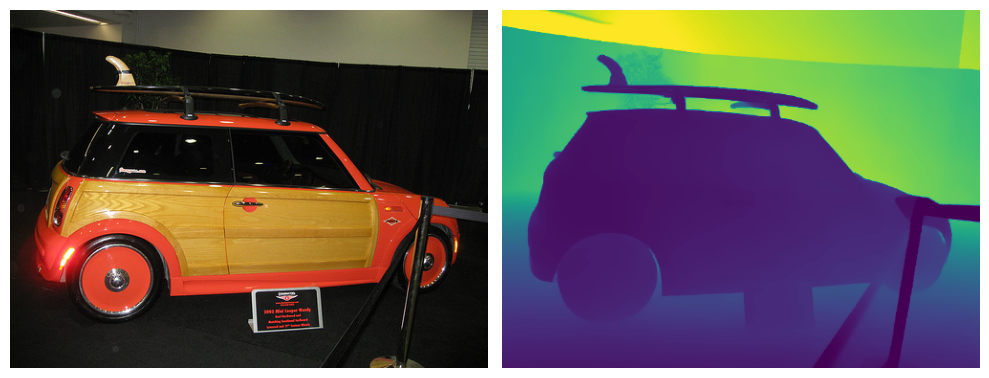
\includegraphics[width=1\linewidth]{./images/Original-vs-Marigold.png}
    \caption{Side-by-side comparison between an original ImageNet RGB image and its estimated depth map using Marigold.}
    \label{fig:imagenet-depth-est-example}
\end{figure}

\subsection{ImageNet 200-class depth}
To further reduce computational overhead while maintaining diversity in object categories, we constructed a 200-class subset of previously mentioned dataset (Imagenet 1k-class depth) by randomly sampling 200 classes from the full 1,000-class set. This subset contains 10,000 images, with 50 images per class. The list of sampled classes can be found in the \href{https://gitlab.com/dariofurlan/vcs-2425/}{Supplementary Material}. This smaller subset is more balanced and allows us to conduct more detailed evaluations by reducing label space complexity while also preserving the large-scale nature of ImageNet.

\subsection{Washington-RGB-D}
The Washington RGB-D Object Dataset \cite{washington-rgbd} is a real-world RGB-D dataset widely used in robotics and object recognition research. It was captured by a Microsoft Kinect sensor and contains 51 categories of common indoor objects (e.g., scissors, cereal boxes, keyboards) with 300 distinct object instances.

The training set includes 207,920 RGB-D frames, and the validation set (which we use in our study) has 41,877 images. Each instance is recorded from three video sequences, with one frame extracted every fifth frame. For each image, the dataset provides aligned RGB, raw depth (in millimeters), segmentation masks, and cropping metadata.

We specifically use the \textit{depthcrop.png} files, which are single-channel, 16-bit depth images. These real depth images were used as-is, with only minor preprocessing. While the dataset was originally intended for object recognition and pose estimation, we repurpose it for our depth-only classification task. 

\subsection{Preprocessing}

Convolutional Neural Networks (CNNs) are typically designed to operate on 3-channel, 8-bit RGB images of fixed dimensions. However, our experiments focus on depth images, which differ significantly in structure and format. Therefore, several preprocessing steps, such as resizing and normalization to standardize input dimensions and pixel value ranges, are necessary to adapt the datasets to the input requirements of standard classification architectures.

% \subsubsection{Depth Estimation for ImageNet}

\subsubsection{Color Mapping Depth Maps for CNNs}
Depth images are single-channel and thus incompatible with CNNs pretrained on RGB data like AlexNet, VGG19, ResNet50 and Inception-v3. To bridge this gap, we convert them into three-channel inputs using perceptually uniform colormaps and a custom stacked encoding. Unlike the commonly used jet (rainbow) colormap, these mappings preserve perceptual ordering and reduce visual artifacts that may impair representation learning \cite{rainbow_harmful}. This process is composed of two main steps:

\begin{itemize}
    \item Normalization: The 16-bit depth values (range: 0-65,535) are scaled down to 8-bit values (range: 0-255) using min-max normalization.
    \item Channel Expansion: We convert the single-channel 8-bit image into a 3-channel image using two main strategies:
    \begin{itemize}
        \item Channel Duplication (Stacking): Simply by replicating the depth channel across all three channels.
        \item Colormap Mapping: We apply perceptually uniform colormaps (Viridis, Plasma, Magma and Grayscale) to produce pseudo-RGB images, allowing us to investigate whether color encoding affects feature extraction as shown in the \autoref{fig:depth-color-mapping-examples}.
    \end{itemize}
\end{itemize}

\begin{figure}[h]
    \centering
    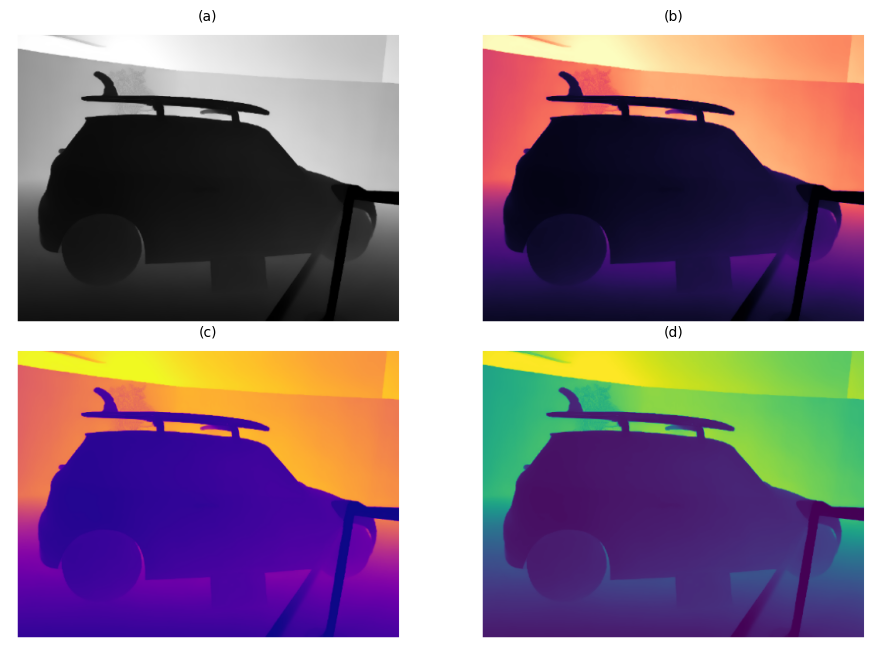
\includegraphics[width=1\linewidth]{./images/stacked-plasma-virdis-and-magma.png}
    \caption{Examples of 8-bit 3-channel depth images obtained through different preprocessing methods: (a) stacked and grayscale, (b) Magma, (c) Plasma, and (d) Viridis colormaps. \\ \textit{Note that grayscale and stacked images are visually similar, as they both represent depth information without color encoding.}}
    \label{fig:depth-color-mapping-examples}
\end{figure}

\subsubsection{Preprocessing the Washington RGB-D Dataset}
The Washington RGB-D dataset already includes 16-bit depth maps captured via Kinect. We applied the same post-processing steps used for ImageNet: 16-bit depth values to 8-bit normalization, and conversion to 3-channel format via channel duplication and colormap mapping. This ensures consistency in input structure across both synthetic and real-world depth data.
